% ===================================================================================================
%                                                 |                                                 |
%                                                 |                                                 |
% -------------------------------------------- SECTION ---------------------------------------------|
%                                                 |                                                 |
%                                                 |                                                 |
% ===================================================================================================
\section{Mathematical framework}\label{sec:transfer_learning}
In this section we model the scaling of energy and time demand that results from the use of a set of several robots performing numerous skills.

% ===================================================================================================
\subsection{Energy and time demand for learning skills}
% ---
\begin{figure}[!ht]
	\centering
	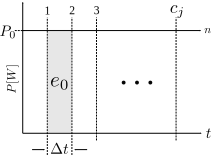
\includegraphics[width=0.9\columnwidth]{fig/power_per_episode.pdf}
	\caption{Power consumption per episode.}
	\label{fig:power_per_episode}
\end{figure}
%---
\begin{tcolorbox}
	\begin{definition}\label{definition:complexity}
		The complexity $c_j$ of a skill $ s_j $  is understood as the number of trial episodes $n$ needed to successfully learn the skill; i.e., all actions and states visited until a stopping criterion is reached. 
	\end{definition}
\end{tcolorbox}
% ---

Consider $P_0$ to be the constant power demand of a given robot during the learning of a skill. Furthermore,% ---
% ---
\begin{tcolorbox}
	\begin{assumption}\label{assumption:time}
		the same amount of time $\Delta t$ is allocated for the execution of each trial episode $n$ (see Fig.~\ref{fig:power_per_episode}).
	\end{assumption}
\end{tcolorbox}
% ---
% ---------------------------------------------------------------------------------------------------
\subsubsection{\textbf{Energy requirement}}
Under Asm.~\ref{assumption:time}, the energy consumption of the $n$-th episode $e_j(n)$ is simply
% ---
\begin{equation}\label{eq:energy_per_episode}
    e_j(n) = \underbrace{P_0\cdot \Delta t}_{\text{constant}} = e_0.
\end{equation}
% ---
Consequently, the energy consumed by a robot learning the skill $ s_j $ is directly proportional to the complexity; i.e.
% ---
\begin{equation}\label{eq:energy_per_skill}
    E_j =\sum_{n=1}^{c_j} e_j(n) = e_0 \cdot c_j.
\end{equation}
% ---
Having $\mathcal{S}$ represent the set of all \emph{to-be-learned} skills, with $|\mathcal{S}| = N_\mathcal{S}$; then, the energy spent on learning $\mathcal{S}$ is
% ---
\begin{equation}\label{eq:total_energy}
	E_{\mathcal{S}} = \sum_{j=1}^{{N_{\mathcal{S}}}} E_j = e_0 \sum_{j=1}^{{N_{\mathcal{S}}}} c_j%N_{\mathcal{T}} \cdot e_0 \cdot c_j 
\end{equation}
% ---
% ---------------------------------------------------------------------------------------------------
\subsubsection{\textbf{Time requirement}}
Similarly, the total time $T_{\mathcal{S}}$ is simply
% ---
\begin{equation}\label{eq:total_energy}
	T_{\mathcal{S}} = \Delta t \sum_{j=1}^{{N_{\mathcal{S}}}} c_j.
\end{equation}
% ---
% ===================================================================================================
\begin{figure}[!t]
	\centering
	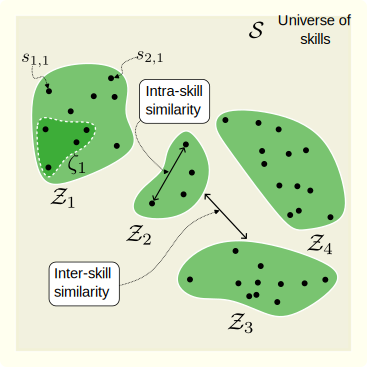
\includegraphics[width=0.9\columnwidth]{fig/skill_similarity.pdf}
	\caption{Similar skills in $\mathcal{S}$ can be grouped into clusters $\mathcal{Z}_k$.}
	\label{fig:skill_similarity}
\end{figure}
\subsection{Similarity and knowledge}
%---
\begin{tcolorbox}
	\begin{assumption}\label{assumption:skill_clustering} When the degree of similarity among a set of skills is comparable, they can be clustered together.
		\end{assumption}
\end{tcolorbox}
% ---
Following Asm.~\ref{assumption:skill_clustering}, let $\mathcal{Z}_k \subset \mathcal{S}$ be a subset of $N_{\mathcal{Z}_k}$ skills that share high similarity; i.e. a \emph{cluster} of skills, see Fig.~\ref{fig:skill_similarity}. Furthermore, consider another set $\mathcal{\zeta}_k \subset \mathcal{Z}_k$ that denotes already learned skills from $\mathcal{Z}_k$. Asm.~\ref{assumption:skill_clustering} implies that the $j$-th skill in the $k$-th cluster $s_{j,k} \in \mathcal{Z}_k$ can always benefit from the knowledge contained in $\mathcal{\zeta}_k$. This implies that the more skills enter $\mathcal{\zeta}_k$, the less knowledge about $ s_{j,k} $ will remain to be learned.

Now, we introduce a function \hl{$\bar{\sigma}_{j,k}\left(n\right)\in [0,1]$ that expresses the knowledge about a skill $s_{j,k} \in \mathcal{Z}_k$ that \textbf{is not} contained in $\mathcal{\zeta}_k$; i.e. $s_{j,k} \notin \mathcal{\zeta}_k$}. The function $\bar{\sigma}_{j,k}(\cdot)$ satisfies:
% ---
\begin{itemize}
	\item $\bar{\sigma}_{j,k}\left(n\right) = 1$, if $\mathcal{\zeta}_k=\emptyset$ or if it does not contain knowledge about the skill $s_{j,k}$
	\item $\bar{\sigma}_{j,k}\left(n\right) = 0$, if \emph{all} the knowledge about skill $s_{j,k}$ is contained in $\mathcal{Z}_k$
\end{itemize} 
\textcolor{red}{Conceptually, $\bar{\sigma}_ {j,k}\left(\cdot\right)$ is the fraction of knowledge from ${\mathcal{Z}_k}$ that remains to be learned.}
% ---
% ---------------------------------------------------------------------------------------------------
\subsubsection{\textbf{Leveraging the acquired knowledge}}
To simplify the analysis, we introduce a fundamental complexity
\begin{tcolorbox}
\begin{assumption}\label{assumption:fundamental_complexity} The fundamental complexity $c_0$ describes the maximum number of episodes required to learn \emph{any} skill.
\end{assumption}
\end{tcolorbox}
% ---
If, in learning a skill $ s_{j,k} $, a robot uses the knowledge contained in $\mathcal{\zeta}_k$; then, two effects take place:
\begin{enumerate}
	\item There is less remaining knowledge and this is reflected in the initial value; i.e. $\bar{\sigma}_{j,k}(0) < 1$
	\item Knowledge is acquisition is expedited 
\end{enumerate}
%associated complexity $ c_{j,k} $ is necessarily smaller than the fundamental complexity $c_{0}$; i.e. $c_{j,k} < c_0~\forall j>1$.
This implies that the remaining knowledge scales down as a function of the number of learned skills $N_{\zeta_k}=|\mathcal{\zeta}_k|$.%, as exemplified in Fig.~\ref{fig:complexity_per_cardinality}. 

%Furthermore, consider the following assumptions
%% ---
%\begin{tcolorbox}
%	\begin{assumption}\label{assumption:skill_clustering} When the degree of similarity among a set of skills is comparable, they can be clustered together.
%	\end{assumption}
%\end{tcolorbox}
%% --- 
%The previous assumption is depicted in Fig.~\ref{fig:incremental_transfer_similarity} where similar skills are grouped together in four different clusters.
\begin{tcolorbox}
	\begin{assumption}\label{assumption:exponential_decrease} The knowledge function $\bar{\sigma}_{j,k}(\cdot)$ has a monotonically decreasing behavior.
	\end{assumption}
\end{tcolorbox} 
% ---
\noindent
An idealization of the behavior described in Asm.~\ref{assumption:exponential_decrease} can be modeled via the linear homogeneous differential equation
% ---
%\begin{subequations}\label{eq:simple_knowledge_dynamics}
%	\begin{alignat}{2}
%		\dot{\bar{\sigma}}_{j,k}\left(n\right) &= -\alpha r f\left(N_{\zeta_k}\right) \bar{\sigma}_{j,k}\left(n\right)\\
%		\bar{\sigma}_{j,k}(0) &= g\left(N_{\zeta_k}\right)
%	\end{alignat}
%\end{subequations}
\begin{subequations}\label{eq:simple_knowledge_dynamics}
	\begin{alignat}{2}
		\dot{\bar{\sigma}}_{j,k}\left(n\right) &= -\alpha f\left(N_{\zeta_k},r\right) \bar{\sigma}_{j,k}\left(n\right)\\
		\bar{\sigma}_{j,k}(0) &= g\left(N_{\zeta_k},r\right)
	\end{alignat}
\end{subequations}

% ---
which is a function of the trial episodes $n$ and is parameterized by the number of already learned skills $N_{\zeta_k}$, the factor $ \alpha>0$ that models the rate at which a robot in isolation learns any given skill and \textcolor{red}{the number $r$ of \textbf{robots exchanging knowledge} about concurrently learned skills}. The solution to \eqref{eq:simple_knowledge_dynamics} is given by
% ---
%\begin{equation}\label{eq:knowledge_exponential_form}
%     \boxed{\bar{\sigma}_{j,k}(n) = g\left(N_{\zeta_k}\right) \left[ \left(e^{-\alpha n}\right) ^{f\left(N_{\zeta_k}\right)}\right]^r \in (0,1]}
%\end{equation}
\begin{equation}\label{eq:knowledge_exponential_form}
	\boxed{\bar{\sigma}_{j,k}(n) = g\left(N_{\zeta_k}, r\right) \left(e^{- \alpha  n}\right) ^{f\left(N_{\zeta_k}, r\right) n} \in (0,1]}
\end{equation}
% ---
and meets the desired behavior, see Fig.~\ref{fig:knowledge_idealization}. The function $f\left(N_{\zeta_k}\right)$ expresses the form in which the learned skills affect the original rate $\alpha$. A possible realization is to make this effect proportional; i.e.
% ---
\begin{equation}\label{eq:f_function}
	f\left(N_{\zeta_k},r\right) = \frac{1}{(1 - \beta_k)}\left( \eta r N_{\zeta_k} + 1 \right),
\end{equation}
% ---
where $\eta$ represents how efficient is the exchange of knowledge from $\zeta_k$ to $s_{j,k}$. Similarly, $g\left(N_{\zeta_k}\right)$ models the change in the initial remaining knowledge that results from $\zeta_k$. Although many potential models might be used, we envision the effect to be of exponential nature; i.e.
% ---
\begin{equation}\label{eq:g_function}
	g\left(N_{\zeta_k},r\right) = (1-\beta_k) e^{-\delta r N_{\zeta_k}},
\end{equation}
%---
again with a term $\delta$ controlling the rate at which the exponential converges as a function of the number of seen skills $N_{\zeta_k}$. In both \eqref{eq:f_function} and \eqref{eq:g_function},   $\beta_k$ is the head start granted by knowledge transfer from other clusters to the skills in $\mathcal{Z}_k$.
\begin{figure}[!t]
	\centering
	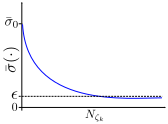
\includegraphics[width=0.8\columnwidth]{fig/knowledge_idealization.pdf}
	\caption{The idealized remaining knowledge to learn a new skill $s_{j,k}$ as a function of the number of learned skills $N_{\zeta_k}$.}
	\label{fig:knowledge_idealization}
\end{figure}
% ---
% ===================================================================================================
\subsection{Knowledge sharing under different learning paradigms}
The following assumptions are analogous to average behavior and imply that a suitable scaling strategy is available and executed.
% ---
\begin{tcolorbox}
	\begin{assumption}\label{assumption:agent_similarity}
		Every agent has the same capabilities and energetic cost.
	\end{assumption}
\end{tcolorbox}
% %---
% \begin{tcolorbox}
% 	\begin{assumption}\label{assumption:skill_clustering} When the degree of similarity among a set of skills is comparable, they can be clustered together.
% 		\end{assumption}
% \end{tcolorbox}
% % ---
\begin{tcolorbox}
	\begin{assumption}\label{assumption:cluster_size}
		Every cluster $\mathcal{Z}_{k}$ contains the same number $N_{\mathcal{Z}} $ of skills.
	\end{assumption}
\end{tcolorbox}
% ---
\begin{tcolorbox}
	\begin{assumption}\label{assumption:cluster_transferability}
		The knowledge transferability between skills is assumed to be equal; therefore, also the transferability between clusters is assumed to be equal.
	\end{assumption}
\end{tcolorbox}
% ---------------------------------------------------------------------------------------------------
\subsubsection{\textbf{Isolated learning (Iso)}} A robot learns each skill in $\mathcal{Z}_k$ one after another from the ground up, disregarding the accumulating knowledge from already learned skills; in other words, this implies that $N_{\mathcal{\zeta}_k} = 0$ in \eqref{eq:knowledge_exponential_form}. Therefore, the energy required by one single robot to learn the skills in the cluster $\mathcal{Z}_k$ is given by
% ---
 \begin{align}
     \begin{split}
       E^{(Iso)}_{\mathcal{Z}_k} &= \sum_{j=1}^{N_{\mathcal{Z}}} E^{(Iso)}_j= N_{\mathcal{Z}_k}  e_{0} \cancelto{c_{0}}{c_{j,k}} = N_{\mathcal{Z}} e_{0}  c_0
     \end{split}
 \end{align}
%-- 
If $\mathcal{S}$ is divided into $\left\lbrace \mathcal{Z}_k \right\rbrace^{N_\mathcal{K}}_{k=1} $ clusters, the total energy to learn the universe of skills is simply
% ---
\begin{equation}
	E^{(Iso)}_{\mathcal{S}} = N_\mathcal{K} N_{\mathcal{Z}} e_{0}  c_0.
\end{equation}
% ---
Notice that using a batch of $m$ robots to learn the same number of skills in parallel does not bring about any energy reductions since
% ---
\begin{equation}
    ^{\lvert \lvert}E^{(Iso)}_\mathcal{S}= \underbrace{m}_{\text{robots}}\cdot \overbrace{\frac{1}{m}E^{(Iso)}_\mathcal{S}}^{\text{energy per robot}} = E^{(Iso)}_\mathcal{S}.
\end{equation}
% ---


%---
% \begin{figure}[!ht]
% 	\centering
% 	\includegraphics[width=0.99\columnwidth]{tex/fig/single_incremental_knowledge.pdf}
% 	\caption{Knowledge sharing in incremental learning. A single agent leverages previously acquired knowledge from other learned skills in $\mathcal{Z}$.}
% 	\label{fig:single_incremental_knowledge}
% \end{figure}

% ---
\begin{figure}[!t]
	\centering
	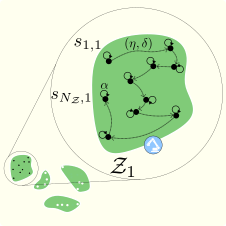
\includegraphics[width=0.9\columnwidth]{fig/intra_skill_learning.pdf}
	\caption{Incremental learning benefits from the high similarity of skills belonging to the same cluster.}
	\label{fig:intra_skill_learning}
\end{figure}
% ---
% ---
\begin{figure*}[!htb]
	\centering
	\hspace*{\fill}
	\subfloat[]{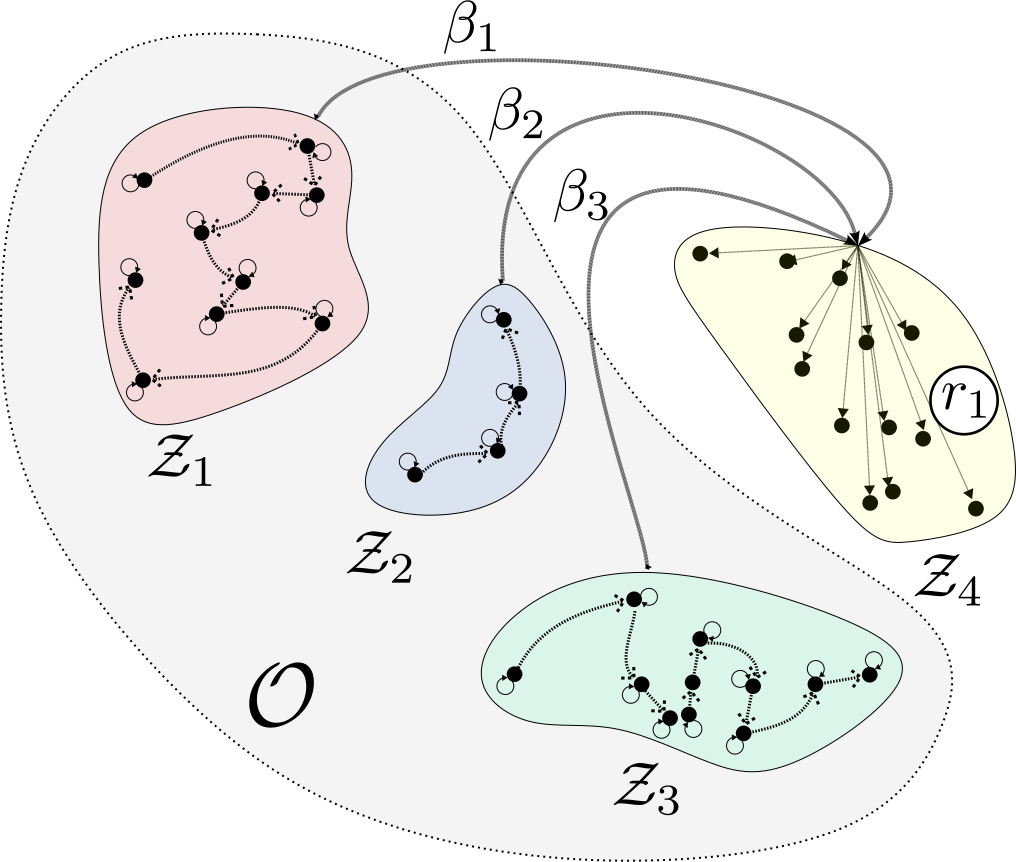
\includegraphics[width= 0.30\textwidth]{fig/cluster_to_cluster_knowledge_transfer.pdf} \label{fig:cluster_to_cluster_knowledge_transfer}}  
	\hfill
	\subfloat[]{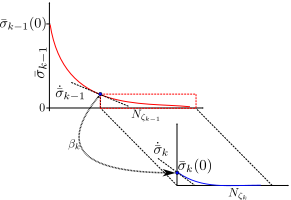
\includegraphics[width= 0.30\textwidth]{fig/effect_transfer_learning.pdf} \label{fig:effect_transfer_learning}}  
	\hfill	
	\subfloat[]{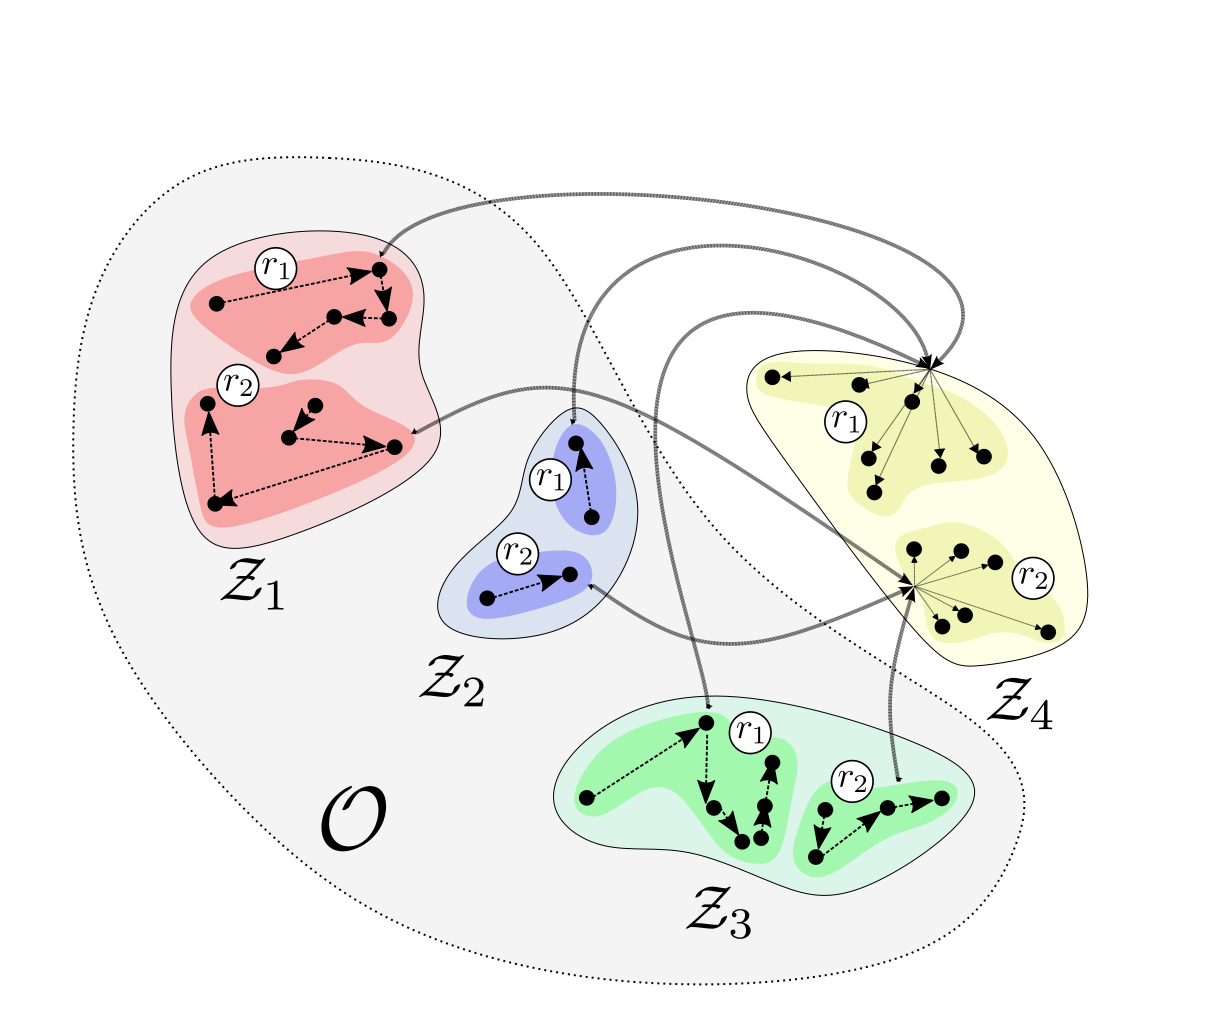
\includegraphics[width= 0.30\textwidth]{fig/cluster_to_cluster_knowledge_transfer_parallel.pdf} \label{fig:cluster_to_cluster_knowledge_transfer_parallel}}
	\hspace*{\fill}
	\caption[] {\label{fig:tranfer_learninhg} Transfer learning. \subref{fig:cluster_to_cluster_knowledge_transfer} Transfer of knowledge from different origin clusters to the target cluster, \subref{fig:effect_transfer_learning} the effect of transfer learning,  \subref{fig:cluster_to_cluster_knowledge_transfer_parallel} using several robots only subdivides the problem.}
\end{figure*}
% ---
% ---------------------------------------------------------------------------------------------------
\subsubsection{\textbf{Incremental learning (I)}}
\textcolor{red}{\textbf{INTRA cluster}}
Referring back to Asm.~\ref{assumption:skill_clustering}, the knowledge from skills belonging to a cluster ${\mathcal{Z}_k}$ can be be leveraged by an agent in virtue of their high similarity. As depicted in Fig.~\ref{fig:intra_skill_learning}, a robot ($r_1$ in this case) learns every skill in $\mathcal{Z}_1$ with a rate $alpha$ ---the self loops--- but also passes the acquired knowledge to the subsequent skills, via the exchange factors $(\eta,\delta)$. Therefore, in incremental learning the knowledge about every new skill gets gradually increased by leveraging previous knowledge, resulting in the expression
% ---
\begin{equation*}\label{eq:remaining_knowledge__IL}
	\bar{\sigma}^{(I)}_{i,j}(n) = e^{-\alpha  \left(\eta N_{\zeta_k}+1\right) n} e^{-\delta N_{\zeta_k}},
\end{equation*}
% ---
which is equivalent to \eqref{eq:knowledge_exponential_form} with $r=1$ since no inter-agent exchange of knowledge occurs and $\beta_k = 0$,¸ as knowledge from other cluster cannot be used. As the complexity $c_{j,k}$ of a skill can also be interpreted as the number of trial episodes such that the remaining knowledge goes below a threshold $\epsilon$; i.e.
% ---
\begin{equation*}
	\bar{\sigma}^{(I)}_{i,j}(n) \rvert_{n \ge c_{j,k}} \leq \epsilon,
\end{equation*}
% ---
then under this scheme the complexity $c_{j,k}$ to learn a new is skill in the cluster results in
%\begin{equation}\label{eq:complexity_IL}
%	c^{(I)}_{j,k} = -\frac{\text{log}(\epsilon)}{\alpha \eta (N_{\zeta_k}+ 1)}.
%\end{equation}
\begin{equation}\label{eq:complexity_IL}
	c^{(I)}_{j,k} = -\frac{\text{log}(\epsilon) - \text{log}(\bar{\sigma}^{(I)}_{j,k}(0))}{\alpha (\eta N_{\zeta_k}+ 1)} = -\frac{\text{log}(\epsilon) + \delta N_{\zeta_k}}{\alpha (\eta N_{\zeta_k}+ 1)}  .
\end{equation}
% ---
The total number of trial episodes $ C_k $ that an agent following an incremental learning strategy needs to learn the $N_{\mathcal{Z}_k}$ skills in a cluster $ \mathcal{Z}_k $ is given by
% ---
\begin{align}\label{eq:total_episodes_incremental}
	\begin{split}
		C^{(I)}_k &= \sum^{N_{\mathcal{Z}}}_{j=1} c^{(I)}_{j,k}.
	\end{split}
\end{align}
If $m$ robots are used in parallel to divide the load of learning the tasks then
% ---
\begin{align}
	\begin{split}
		{}^{\lvert \rvert}C^{(I)}_k &= m\sum^{\frac{N_{\mathcal{Z}}}{m}}_{j=1} c^{(I)}_{j,k}.
	\end{split}
\end{align}
In essence, using $m$ robots without exchanging knowledge only subdivides the learning in every cluster into $m$ smaller problems without adding any additional benefit to the rate at which knowledge is acquired. 

\subsubsection{\textbf{Transfer learning (TL)}}
\textcolor{red}{\textbf{INTER cluster}}
Considering $\mathcal{K} = \{ \mathcal{Z}_k \}^{N_\mathcal{K}}_{k=1}$ to be the set of all available skill clusters (see Fig.~\ref{fig:cluster_to_cluster_knowledge_transfer}), TL represents the exchange of knowledge from the skills learned in different \emph{origin} clusters $\mathcal{O} = \{ \mathcal{Z}_1,\mathcal{Z}_2,\ldots,\mathcal{Z}_{k-1} \}$ to the skills that will be learned in a \emph{destination} cluster $\mathcal{Z}_k$. Concretely, the effect that TL has on the skills of the destination cluster is the reduction of the initial remaining knowledge and the initial collection rate for all the skills in the cluster via the parameter $\beta_c$ in \eqref{eq:knowledge_exponential_form}, 
%Referring to \eqref{eq:simple_knowledge_dynamics}, it means that its initial condition $\bar{\sigma}_{j,k}(0)$ will be reduced (Fig.~\ref{fig:effect_transfer_learning}). The TL effect can be modeled as follows
%% ---
%\begin{equation}\label{eq:tl_initial_condition}
%	\bar{\sigma}^{(T)}_{j,k}(0) = 1 - \sum\limits_{c = 1}^{k-1}\beta_{c} \left( 1 - \bar{\sigma}_{c} \right),~\bar{\sigma}_{c=0} = 1
%\end{equation}
%% ---
%Implying that the remaining knowledge under transfer learning is
%% ---
%\begin{align}
%	\begin{split}
%		\bar{\sigma}^{(T)}_{j,k} 
%		&= \underbrace{\left[1- \sum\limits_{c = 0}^{k-1}\beta_{c} \left( 1 - \bar{\sigma}_{c} \right)\right]}_{\text{Transferred knowledge}} e^{-\alpha \left(N_{\zeta_k}+1\right) n}
%	\end{split}
%\end{align}
%% ---
where $0<\beta_{c} < 1$ is the transfer coefficient from the different origin clusters $\mathcal{Z}_{c}$ to the target cluster $\mathcal{Z}_{k}$\footnote{\textcolor{red}{Once again, since there is no inter-agent exchange of knowledge, $ r = 1 $ in this case.}}. Asm.~\ref{assumption:cluster_transferability} implies that
% ---
%\begin{equation}
%	\sum\limits_{c=0}^{k-1}\beta_{c} \leq 1;
%\end{equation}
\begin{equation}
	\sum\limits_{k=1}^{N_\mathcal{K}}\beta_{k} \leq 1
\end{equation}
% ---
and
% ---
% \begin{equation}
	%     \beta_{k_O} = \frac{1}{\text{max}\left(\left\lvert \mathcal{K} \setminus k_{T} \right\rvert,1\right)}
	% \end{equation}
%\begin{equation}
%	\beta_{c}=
%	\begin{cases}
%		1, & \text{if $\mathcal{O}  = \emptyset$}.\\
%		\frac{c}{N_\mathcal{Z}}, & \text{otherwise}.
%	\end{cases}
%\end{equation}
\begin{equation}
	\beta_{k}= \frac{k-1}{N_\mathcal{K}}.
\end{equation}
% ---
Notice that this choice of $\beta_k$ requires that all the skills from the origin clusters were learned. The remaining knowledge when transfer and incremental learning are used in conjunction is
% ---
\begin{equation*}\label{eq:remaining_knowledge__ITL}
	\bar{\sigma}^{(I)}_{k,k}(n) = \left(1- \beta_k\right) e^{-\alpha  \left[\frac{ \left(\eta N_{\zeta_k}+1\right)}{1 - \beta_k}\right] n} e^{-\delta N_{\zeta_k}},
\end{equation*}
% ---
Similar to incremental learning the complexity to learn a skill in transfer learning is
\begin{equation}\label{eq:skill_complexity_TL}
	c^{(IT)}_{j,k} = -\frac{1 - \beta_{k}}{\alpha (\eta N_{\zeta_k}+ 1)}\left[\text{log}(\epsilon) + \delta N_{\zeta_k} - \text{log}(1 - \beta_{k})\right].
\end{equation}
% ---

Similar to incremental learning the total number of episodes  $ C_k $ that an agent requires to learn the $N_{\mathcal{Z}_k}$ skills in	 merely their sum
% ---
\begin{align}\label{eq:total_episodes_transfer}
	\begin{split}
		C^{(IT)}_k &= \sum^{N_{\mathcal{Z}}}_{j=1} c^{(T)}_{j,k}.
	\end{split}
\end{align}
If $m$ robots are used in parallel to divide the load of learning the tasks then
% ---
\begin{align}
	\begin{split}
		{}^{\lvert \rvert}C^{(IT)}_k &= m\sum^{\frac{N_{\mathcal{Z}}}{m}}_{j=1} c^{(IT)}_{j,k}.
	\end{split}
\end{align}
% ---
The effect of this having m robots learning in parallel is depicted on Fig.~\ref{fig:cluster_to_cluster_knowledge_transfer_parallel}, where two robots $ r_1$ and $r_2$ learn skills in four different clusters. The shaded areas are the subclusters of skills learned by each robot. Since they do not share knowledge between them, each robot has access only to the knowledge it has collected and cannot benefit from one another. 

% ---------------------------------------------------------------------------------------------------
\subsubsection{\textbf{Collective learning (C)}}
% ---
\begin{figure}[!th]
	\centering
	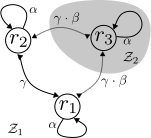
\includegraphics[width=0.7\columnwidth]{fig/cl_example_figure.pdf}
	\caption{Exchange of knowledge between robots enables collective learning.}
	\label{fig:cl_example_figure}
\end{figure}
% ---
The key aspect in collective learning is that the exchange of knowledge between a batch of robots $\left \lbrace r_i \right \rbrace^m_{1}$ is now enabled. Fig.~\ref{fig:cl_example_figure} illustrates the concept, the self loop represents the dynamics of a single robot learning, expressed by \eqref{eq:simple_knowledge_dynamics}. The exchange of knowledge is represented via the cross-couplings weighted by a parameter $\gamma$ that models how efficient is the bidirectional pairwise knowledge exchange. Similar to transfer learning, if two robots exchange knowledge about skills with low similarity (i.e. skills in different clusters), then $\gamma$ is scaled by the inter-cluster transferability  parameter $\beta$. To account for the couplings \eqref{eq:simple_knowledge_dynamics} is extended to 
% ---
%\begin{subequations}\label{eq:collective_knowledge_dynamics}
%	\begin{alignat}{2}
%		\dot{\bar{\bm{\sigma}}}_{j,k}\left(n\right) &= -\bm{A} r \left(N_{\zeta_k} + 1\right) \bar{\bm{\sigma}}_{j,k}\left(n\right)\\
%		\bar{\bm{\sigma}}^{(T)}_{j,k}(0) &= 1 - \sum\limits_{c = 1}^{k-1}\beta_{c} \left( 1 - \bar{\bm{\sigma}}_{c} \right),~\bar{\bm{\sigma}}_{c=0} = 1,
%	\end{alignat}
%\end{subequations}


\begin{subequations}\label{eq:collective_knowledge_dynamics}
	\begin{alignat}{2}
		\dot{\bar{\bm{\sigma}}}^{(C)}_{j,k}\left(n\right) &= \left[-\alpha  f\left(N_{\zeta_k},r\right) \bm{I} + \gamma \bm{A} \odot \bm{B}  \right] \bar{\bm{\sigma}}_{j,k}\left(n\right)\\
		\bar{\bm{\sigma}}^{}_{j,k}(0) &= g\left( N_{\zeta_k}, r\right) \bm{I},
	\end{alignat}
\end{subequations}
with $\bar{\bm{\sigma}}^{}_{j,k} \in \mathbb{R}^r$ and $\bm{A} \in \mathbb{R}^{r \times r}$ being the zero-diagonal symmetric adjacency matrix whose entry $(\bm{A})_{i,j} = 1$ if robot $i$ exchanges knowledge with robot $j$ an $(\bm{A})_{i,j} = 0$ if it does not. The term $\gamma \in \mathbb{R}_+ $ weighs the knowledge exchange strength among robots. Furthermore, since robots may learn skills in different clusters at the same time, the matrix $\bm{B}$, whose entries are $\left(\bm{B}\right)_{i,j} \in \left \lbrace 1, 1/N_\mathcal{K} \right \rbrace$, scale down the knowledge contributions between robots from different clusters.

Given the dynamics matrix of the collective system
% ---
\begin{equation}
	\bar{\bm{A}}\left(N_{\zeta_k}\right) =-\alpha  f\left(N_{\zeta_k},r\right) \bm{I} + \gamma \bm{A} \odot \bm{B} 
\end{equation} 
% ---
it can be proven that there is a coupling strength $\gamma$ that ensures that the remaining knowledge for all skills converges asymptotically to zero. Notice that \eqref{eq:collective_knowledge_dynamics} is a skill-varying system by virtue of the dependence of $\bar{\bm{A}}$ on the number of seen skills $N_{\zeta_k}$.

\TODO \textcolor{red}{is there an approximation of the convergence rate of all the skills?}


% The term $a$ is defined as
%\begin{equation}
%			\dot{\bar{\sigma}}_{j,k}\left(n\right) = -\alpha r f\left(N_{\zeta_k},r\right) \bar{\sigma}_{j,k}\left(n\right) = a\left(N_{\zeta_k}\right)\bar{\sigma}_{j,k}\left(n\right)\\
%\end{equation} 


%For the system \eqref{eq:collective_knowledge_dynamics} to be \emph{connectively stable}\cite{Pirani2014Stabilitydynamicalsystems}, the coupling parameter $\gamma$ needs to fulfill the following condition
%% ---
%\begin{equation}
%	\gamma\left( N_{\zeta_k}\right)  < - \frac{1}{\lambda_{\text{max}}\left(\bm{A}\right)} a\left( N_{\zeta_k}\right)
%\end{equation}
%% ---
%\important{Is this condition true?´^}
%\begin{subequations}\label{eq:collective_knowledge_dynamics}
%	\begin{alignat}{2}
%		\dot{\bar{\bm{\sigma}}}^{(C)}_{j,k}\left(n\right) &= -\bm{A}(\alpha,  \beta, \gamma) r f\left(N_{\zeta_k}; \beta, \eta \right) \bar{\bm{\sigma}}_{j,k}\left(n\right)\\
%		\bar{\bm{\sigma}}^{}_{j,k}(0) &= g\left( N_{\zeta_k}; \beta, \delta \right),
%	\end{alignat}
%\end{subequations}
% ---
%with $\bm{A} \in \mathbb{R}^{r \times r}$ defined as
%% ---
%\begin{equation}
%	\bm{A} = \begin{bmatrix} 
%		\alpha_1 & (\beta)\gamma_1  & \dots   & \gamma_{r-1}\\
%		(\beta)\gamma_1 & \alpha_2  &         &  \\
% 		\vdots &         & \ddots  & \vdots\\
%		\gamma_{r-1} & \dots   &         & \alpha_r 
%	\end{bmatrix}.
%\end{equation}
%% ---
%The coupling terms $\gamma_i < \alpha_i$ model the knowledge exchange rate between robots. For simplicity we let $\alpha_1=\dots=\alpha_r=\alpha$ and $\gamma_1=\dots=\gamma_{r-1}=\gamma$.
% ---


% ===================================================================================================
\subsection{The effects of the different paradigms}
To show what is the effect of the different learning paradigms consider a scenario in which the skill fundamental complexity is $c_0=100$ episodes with $N_\mathcal{S}= 512$  skills are divided into $N_\mathcal{K}=4$ clusters of $N_\mathcal{Z} = 128$ skills each. Additionally, we consider that $m=32$ robots are available to learn the skills and that a skill is considered learn once the remaining knowledge goes below $\epsilon = 0.01$. In this scenario the robots are used to learn in parallel the skills of each cluster in succession. The remaining parameters are selected as follows;
\begin{itemize}
	\item $\alpha =  0.0461$
	\item $\delta =  0.0360$
	\item $\eta= 0.1$
\end{itemize} 
The skills learned per robot are shown in Fig.~\ref{fig:collective_learning}, notices that as expected, since incremental learning does not benefit from knowledge from other clusters the robot needs to start accumulating knowledge from the beginning every time it moves to a different cluster. This is not the case in transfer learning, as the more cluster the robot has visited the faster a new skill is learned. The speed of knowledge collection is exponentiated with collective learning thanks to the exchange of knowledge among robots. 
%---
\begin{figure*}[!t]
	\centering
	\hspace*{\fill}
	\subfloat[]{\includegraphics[width= 0.95\textwidth]{fig/dynamics_incremental_learning.pdf} \label{fig:dynamics_incremental_learning}}  
	\hspace*{\fill}
	\\
	\hspace*{\fill}
	\subfloat[]{\includegraphics[width= 0.95\textwidth]{fig/dynamics_incremental_transfer_learning.pdf} \label{fig:dynamics_incremental_transfer_learning}}  
	\hspace*{\fill}
	\\
	\hspace*{\fill}
	\subfloat[]{\includegraphics[width= 0.95\textwidth]{fig/dynamics_collective_learning.pdf} \label{fig:dynamics_collective_learning}}
	\hspace*{\fill}
	\caption[] {\label{fig:collective_learning} Scenario 1: the skills of each cluster are learned by the $ m$ robots in succession.  \subref{fig:dynamics_incremental_learning} incremental learning,  \subref{fig:dynamics_incremental_transfer_learning} incremental + transfer learning, \subref{fig:dynamics_collective_learning} collective learning.}
\end{figure*}
% ---
To assess how the number of robots affects the total number of trial episodes required to learn all the $N_\mathcal{S}$ skills we use the same parameters as before but vary the number of robots in $m \in \left \lbrace 2,4,8,16,32,64\right \rbrace$. Additionally we considered an additional collective learning scenario in which, unlike the previous case, the total number of available robots is distributed equally among the clusters to benefit from transfer learning at an earlier time during learning. The results are shown in Fig.~\ref{fig:total_episodes_per_n_robots}. 
\begin{figure}[!th]
	\centering
	\includegraphics[width=0.9\columnwidth]{fig/total_episodes_per_n_robots.pdf}
	\caption{Total number of episodes to learn the universe of skills as a function of the available robots.}
	\label{fig:total_episodes_per_n_robots}
\end{figure}




